% !TEXroot=main.tex
\section{Kartierung}
{
	Bevor der Roboter sich autonom Bewegen kann, muss dieser seine Umgebung erst kennen. Dafür wird von dieser eine Karte erstellt, auf welche später zurückgegriffen werden kann.
	\subsection{Kartierung mit Hilfe des LiDAR-Sensors}
	{
		Die Kartierung erfolgt mithilfe der Daten des LiDAR-Sensors. Dieser misst den Abstand des Roboters in verschiedene Richtungen punktartig. \newline  
		
		\begin{figure}[H]
			\captionsetup{width=.8\linewidth}
			\centering
			\begin{subfigure}[h]{.33\linewidth}
				\centering
				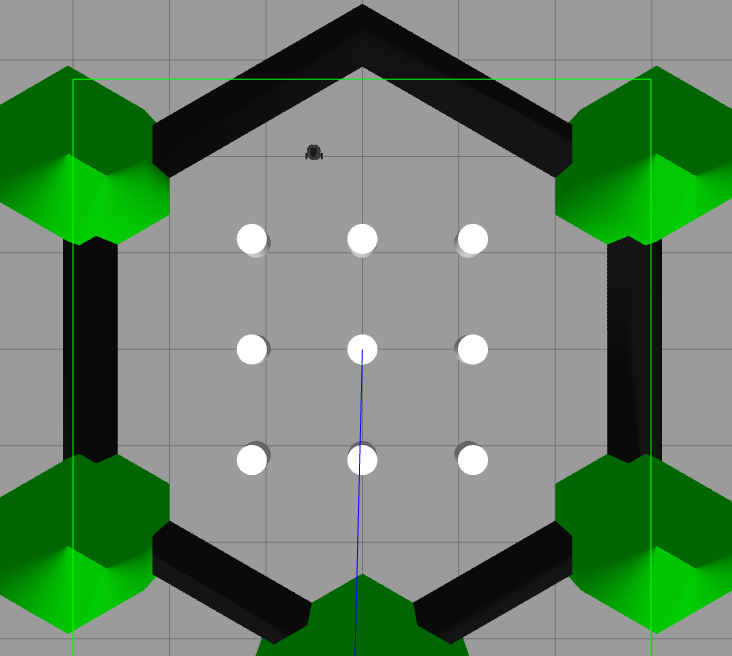
\includegraphics[scale=0.6, height =5cm]{Bilder/virtualmap_world_gazebo.png}
				\subcaption{Roboter (zentriert im oberen Drittel) in einer virtuellen Umgebung}
				\label{pic:virtworldgazebo}
			\end{subfigure}%
			\qquad % erzeugt etwas Abstand
			\begin{subfigure}[h]{.33\linewidth}
				\centering
				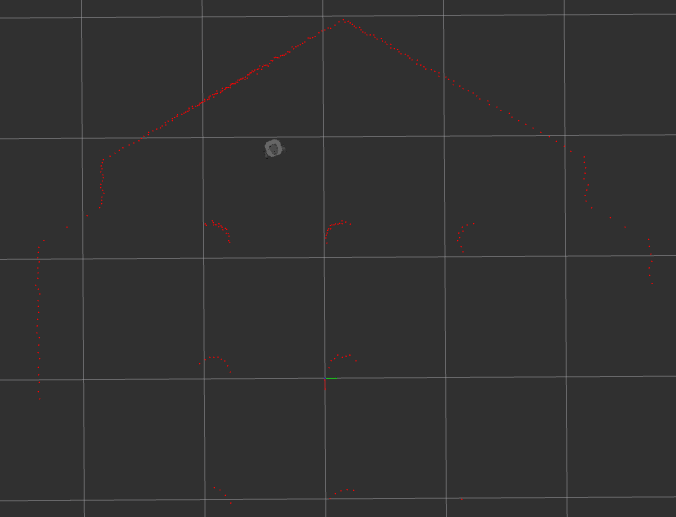
\includegraphics[scale=0.6, height =5cm]{Bilder/virtualmap_world_rviz.png}
				\subcaption{Momentaufnahme der des LiDAR-Sensors gemessenen Punkte (Rot)}
				\label{pic:virtworldlaserrviz}
			\end{subfigure}
			\caption{Eine virtuelle Umgebung und der dazugehörige LiDAR-Scan}
			\label{pic:virtualworld}
		\end{figure}
	
		Links erkennt man eine mit Gazebo simulierte Welt, in welcher sich der Roboter befindet, wobei er von Objekten (Säulen, Mauern) umgeben ist. Das rechte Bild ist ein Ausschnitt aus dem vorher erwähnte Programm Rviz, welches die durch den LiDAR-Sensor gemessene Punkte rot darstellt. Es ist zu erkennen, dass das Verbinden der Roten Punkte auf die Ursprüngliche Umgebung schließen lässt. Je näher der Roboter an einem Objekt ist, desto mehr Punkte befinden sich an dessen Stelle
		
		Zwar gibt eine Messung von einem Standpunkt einen akzeptablen Überblick, so werden jedoch viele Messungen von verschiedenen Stellen benötigt. Durch die Positionsänderung (\emph{siehe Positionierung}) kann errechnet werden wo neue Messpunkte im Vergleich zu alten Messpunkten liegen. Diese Positionierung der Punkte relativ zueinander wird schlussendlich zu einer Karte, wobei viele Messungen nötig sind. Da die Karte jedoch nur aus Punkten besteht, muss der Roboter diese noch interpretieren, sodass viele linear angeordnete Punkte z.B. als Wand interpretiert werden.
		
		Um eine komplette Karte zu erhalten, bewegt sich der Roboter durch die ihm noch unbekannte Welt, bis er eine Region durch genug Messpunkte Kartographiert hat und sich nun in Richtung einer ihm unbekannteren Region bewegen kann. Da der Roboter durch den LiDAR-Sensor konstant seine Umgebung misst, kann die Karte konstant verändert werden, vor allem, wenn der Roboter sich in Richtung weniger erforschte Gebiete bewegt.
		
		Während des Anfangs des Projektes wurde der Roboter noch mit Hilfe der Tastatur an einem Rechner oder über einen Logitech-Controller Gesteuert. Danach wurde daraus jedoch eine autonome Navigation, meist in Richtung von Gebieten, welche weniger erforscht sind. 
		
		Die Kartierung erfolgt mit Hilfe des \emph{GMapping}-Algorithmus. Dieser schaut sich die gescannten Laserdaten der \emph{sensor\textunderscore msgs/LaserScan}-Topic an und veröffentlicht drei Datenarten.
		\begin{enumerate}
			\item ein "Occupancy-Grid": 2D-Karte. Jeder Ort (Pixel) hat einen Ja/Nein Wert, welcher beschreibt, ob sich an der Position ein Objekt befindet oder nicht
			\item Entropie (Sicherheit über die Erkenntnis verschiedener Punkte: unsichere Punkte werden wahrscheinlicher geändert)
			\item Metadaten über die Karte.
		\end{enumerate}
		
		Durch die Kartierung dieses Algorithmus wird aus den einzelnen Laserscan-Daten nun eine Karte. Dies wird in den unteren Abbildungen dargestellt. Hierbei handelt es sich um die Kartierung der in Abbildung \ref{pic:virtworldgazebo} gezeigten Umgebung. Schwarze Punkte wurden als Hindernis erkannt, graue Stellen sind hindernisfreie Punkte. Die durch den LiDAR-Sensor gemessenen Punkte werden in grüner Farbe über die Karte gelegt. In Abbildung \ref{pic:mapping_smpl_2} und \ref{pic:mapping_smpl_3} ist zu erkenne, dass schwarze Punkte nicht direkt mit Gemessenen Punkten des Lasers (grün) übereinstimmen. Dies liegt zum einen darin, dass die Berechnung der Karte Zeit benötigt, weshalb die Punkte noch verarbeitet werden, sowie daran, dass die Aktualisierungsrate der Karte eingestellt werden kann. Während intuitiv eine schnelle Aktualisierungsrate sinnvoll wirkt, ist eine zu hohe Rate nachteilig, da viel Leistung benötigt wird und mehr Fehler gemacht werden, da ungenaue Messpunkte zu schnellen Schlüssen auf der Karte führen. Bei einer längeren Zeitdauer zwischen Kartenaktualisierungen können nämlich mehr gemessene Punkte in Betracht gemessen werden.
		
	
		\begin{figure}[H]
			\captionsetup{width=.8\linewidth}
			\centering
			\begin{subfigure}[h]{.33\linewidth}
				\centering
				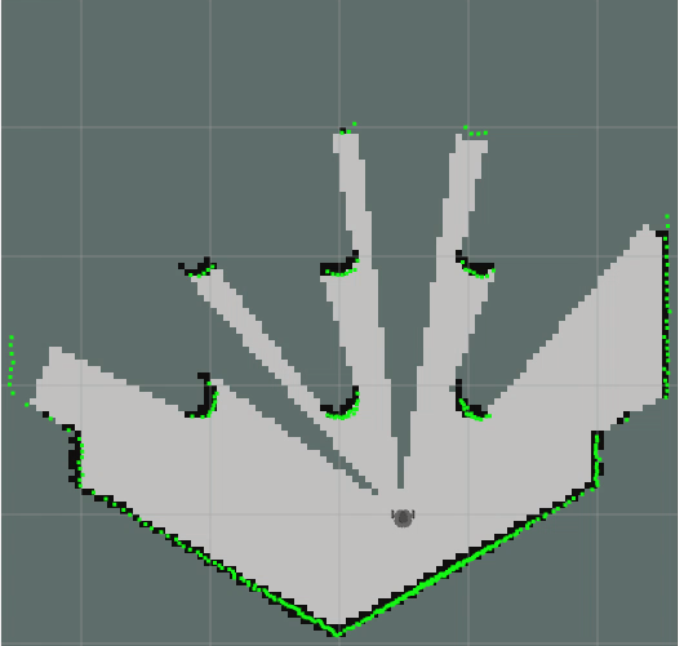
\includegraphics[scale=0.6, height =5cm, width=5cm]{Bilder/mapping_smpl_1.png}
				\subcaption{Kartierung am Anfangspunkt}
				\label{pic:mapping_smpl_1}
			\end{subfigure}%
			\qquad % erzeugt etwas Abstand
			\begin{subfigure}[h]{.33\linewidth}
				\centering
				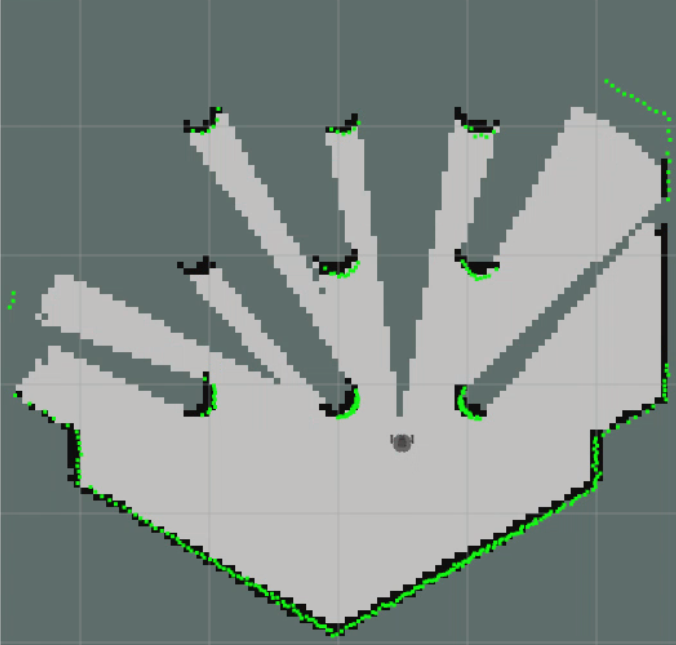
\includegraphics[scale=0.6, height =5cm, width=5cm]{Bilder/mapping_smpl_2.png}
				\subcaption{Kartieruing nach erster Bewegung (nach oben)}
				\label{pic:mapping_smpl_2}
			\end{subfigure}\hfill
			\begin{subfigure}[h]{.33\linewidth}
				\centering
				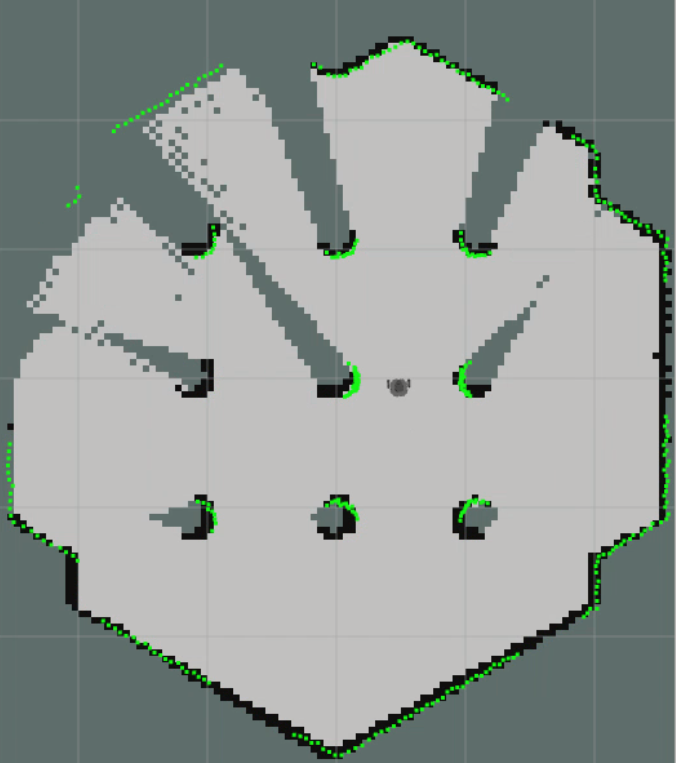
\includegraphics[scale=0.6, height =5cm, width=5cm]{Bilder/mapping_smpl_3.png}
				\subcaption{Kartierung nach weiterer Bewegung}
				\label{pic:mapping_smpl_3}
			\end{subfigure}%
			\qquad % erzeugt etwas Abstand
			\begin{subfigure}[h]{.33\linewidth}
				\centering
				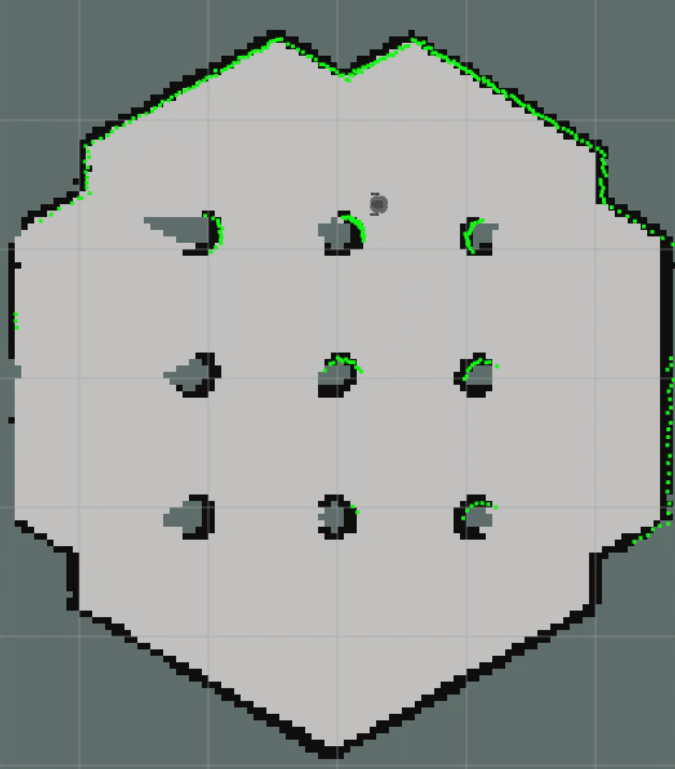
\includegraphics[scale=0.6, height =5cm, width=5cm]{Bilder/mapping_smpl_4.png}
				\subcaption{Kartierung nach Erreichen des oberen Endes}
				\label{pic:mapping_smpl_4}
			\end{subfigure}%
			\caption{Kartierung einer virtuellen Umgebung}
			\label{pic:mapping_smpl}
		\end{figure}
	}
	\subsection{Implementierung}
	{
		Um die Kartierung vor zu nehmen, wird der GMapping, welcher bereits ausgeführt wurde, genutzt. Jedoch müssen einige Parameter angepasst werden, da die Kartierung innerhalb des Labyrinths auf vergleichbar kleinem Raum geschieht. Zuerst wird die Frequenz erhöht, sodass die Karte häufiger, basierend auf den neuen Messdaten, geändert bzw. erneuert wird. Dies wird durch den Parameter $map_update_interval$ bestimmt, welcher auf $6$ gesetzt wird (niedrigerer Wert = niedrigere Periodendauer, woraus eine höhere Frequenz folgt). Gleichzeitig ist zu beachten, dass sich der Roboter auch schnell drehen bzw. bewegen kann. Deshalb müssen Parameter angepasst werden, welche beschreiben, nach welcher zurückgelegten Distanz bzw. Drehung die Karte ebenfalls erneuert wird. Beide Werte werden vergleichsweise niedrig gesetzt, damit die Karte, vor allem bei höheren Geschwindigkeiten oder Drehungen, häufig aktualisiert wird, damit inkorrekte Neupositionierungen oder gar falsche Annahmen über die Umgebung verhindert werden. Dazu wird der $linearUpdate$ Parameter auf $0.05$ und der $angularUpdate$ Parameter auf $0.05$ gesetzt.
		
		Durch den unteren Befehl wird der \emph{GMapping} - Node gestartet.
		\begin{lstlisting}
roslaunch turtlebot3_slam turtlebot3_slam.launch slam_methods:=gmapping
		\end{lstlisting}

	}	

	\subsection{Karten speichern}
	{
		Um einen Raum nicht jedes mal erneut kartieren zu müssen, können Karten auch gespeichert werden. Dafür wird das \emph{map\tus server} - Paket verwendet. Dieses ermöglicht durch den Befehl 
		\begin{lstlisting}
rosrun map_server map_saver -f *path*
		\end{lstlisting}
	das Speichern von erstellten Karten, wobei \emph{*path*} durch Speicherort und Dateinamen ausgetauscht werden muss. Mit Hilfe des Befehls
		\begin{lstlisting}
rosrun map_server map_server  *path.yaml*
		\end{lstlisting}
	kann eine Karte veröffentlicht (gepublished) werden, woraufhin sie für andere Nodes frei verfügbar ist. Auch hier muss \emph{*path*} druch den Pfad der Datei, gefolgt von dem Dateinamen mit der \emph{.yaml} - Endung, ersetzt werden.
	}
}